% !TEX root = ../../main.tex

\section{Energetics of adsorption}

\subsection{Forces involved in adsorption}\label{calo:forces}

From a classical molecular point of view, we can define the
guest-host and guest-guest interactions as a sum of several
components with distinct physical meaning.

\begin{equation}\label{calo:eqn:interactions}
	\Phi_t = \Phi_{R} + \Phi_{D} + \Phi_{C} + \Phi_{I}
\end{equation}

The first two types of interaction, namely short range
electrostatic repulsion between the electron clouds of
neighbouring atoms \(\Phi_{R}\) and long range dispersion \(\Phi_{D}\) arising from
incidental short-lived partial charges are common to all
atoms, and can therefore be called ``non-specific''. Such
interactions are commonly modelled through the use of a
Lennard-Jones type potential function.

\begin{equation}\label{calo:eqn:lennard-jones}
	V_\text{LJ} = 4\varepsilon \left[ \left(\frac{\sigma}{r}\right)^{12} - \left(\frac{\sigma}{r}\right)^6 \right]
\end{equation}

The latter two types, Coulombic interactions \(\Phi_{C}\) and induction
interactions \(\Phi_{R}\) arise from permanent charges and multipoles in the
system. Coulombic interactions are attraction and repulsion
interactions between charges such as molecular ions, permanent
dipoles and quadrupoles.
Induction, also known as polarization or Debye forces, is the interaction
between a charged particle or a multipole with the induced multipole
in a non-charged system. The ease with which a charge can induce such an 
interaction in a molecule is termed polarizability. These interactions
can be referred to as ``specific''.

In the standard definition of adsorption, only
Van-der-Waals forces are said to account for the interactions between
the guest and the host. However, depending on the
systems involved, other types of interactions such
as hydrogen bonding, electron sharing, stacking or \( \pi \) interactions
may also play a role in the overall strength of the guest-host
attraction.

The total interactions can also be broken down as contributions
from adsorbate-adsorbent interactions and guest-guest interactions.
If changes in the adsorbent occur as a result of adsorption,
a host-host or self-potential interaction should be considered.
The guest-host interaction can be assumed constant for a homogeneous
surface or a function of coverage, in the case of a
heterogeneous surface.

\subsection{Adsorption thermodynamics}

As mentioned in the previous section, adsorption
is a consequence of intermolecular attraction between the
material surface and the molecules of the fluid. The sum of
all interactions accounts for the depth of the potential
well and therefore for the energy corresponding to the
process. As this energy is net positive, adsorption is an
overall exothermic phenomenon.

However, in order to make the transition from a molecular
viewpoint to a macroscale bulk fluid representation of
adsorption, the a thermodynamic description of the adsorbed
phase of the process must be performed.

\subsubsection{The Gibbs surface excess approach}

A description of the adsorbed phase can be made through
expressing the change in density or concentration of fluid
from the adsorbent surface to the bulk phase. The density
has a maxima in the immediate zone close to the surface, and then
decreases until it reaches the density of the bulk fluid.
However, when defined as such, the boundary between the
two phases is difficult to pinpoint.
Therefore, in most cases it is useful to employ the concept
of the Gibbs dividing surface.

\begin{figure}[htb]
	\centering

	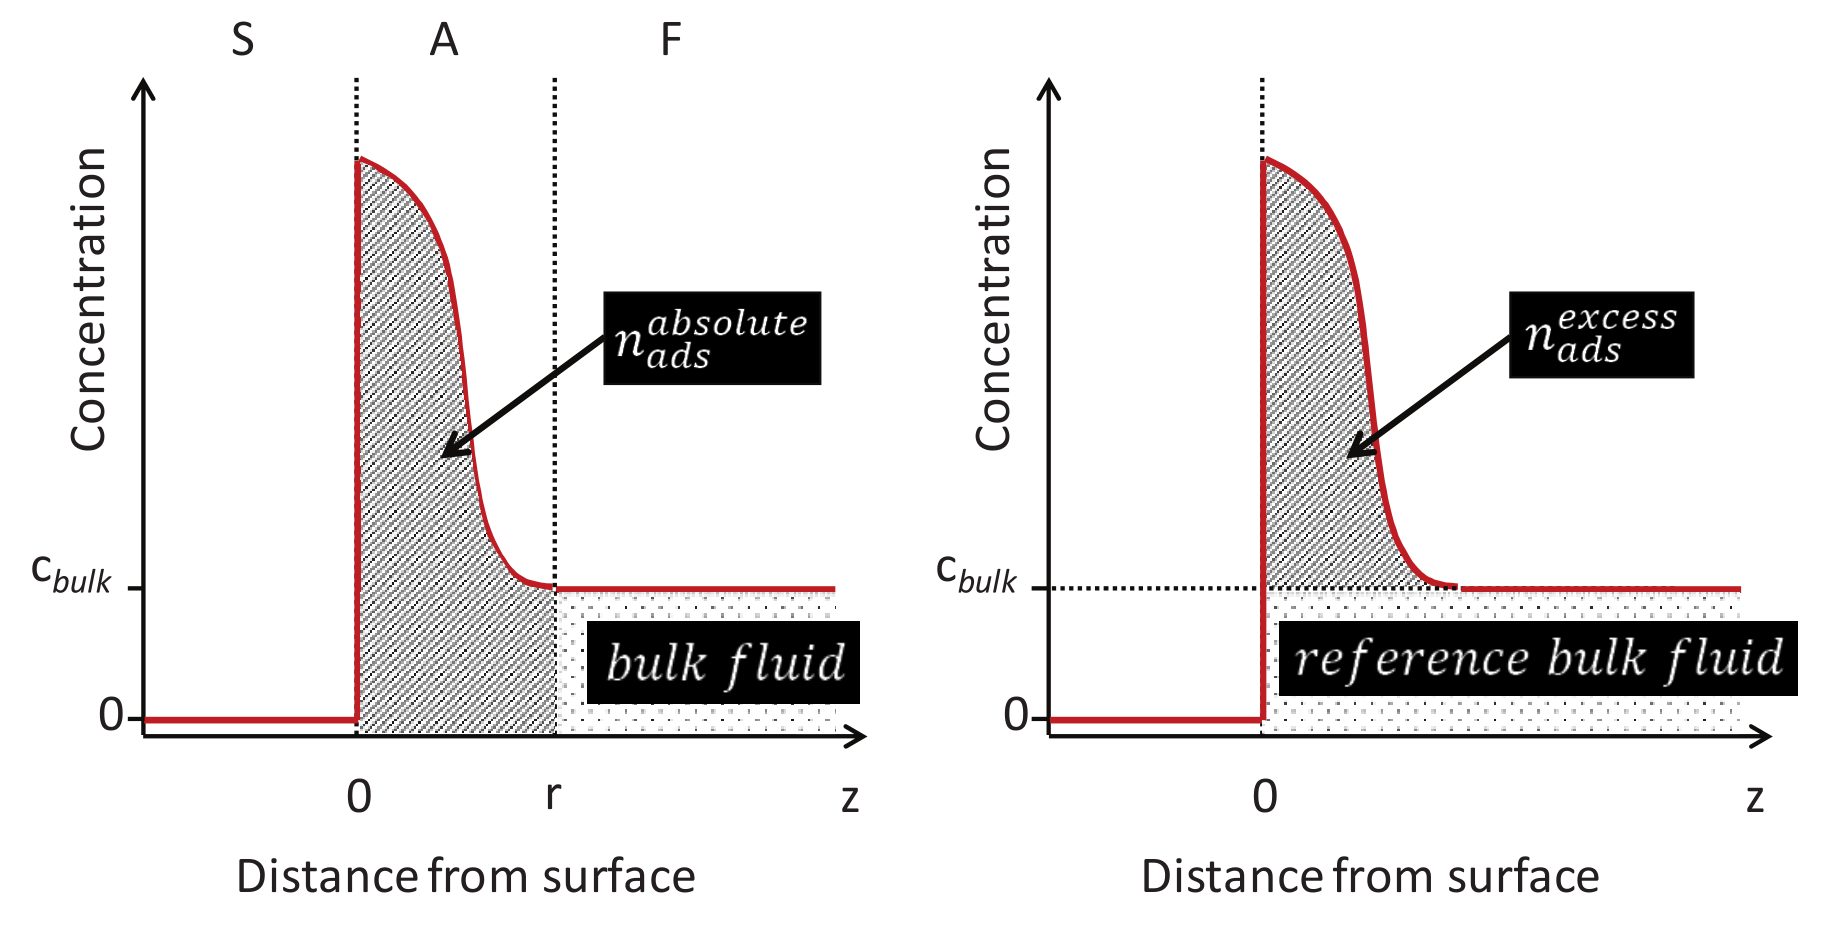
\includegraphics[width=\linewidth]{gibbs-surface}
	\caption{
		Representation of the adsorbed and bulk phases according to
		the (left) layer model and the (right) Gibbs dividing surface
		approach. Adapted from \citeauthor{rouquerolAdsorptionPowdersPorous2013}%
		\cite{rouquerolAdsorptionPowdersPorous2013}.
	}%
	\label{calo:fig:gibbs-surface}

\end{figure}

This approach describes the adsorbed phase only in terms
of an \textit{excess} from the properties of the bulk phase.
As represented in \autoref{calo:fig:gibbs-surface}, the total
amount adsorbed can be defined as:

\begin{equation}
	n_{ads}^{a} = A \int_0^r c\ dz
\end{equation}

The imaginary Gibbs dividing surface is usually placed parallel to
the real surface of the adsorbent and in the resulting system, the
concentration of the adsorbent in the adsorbed phase are
expressed as an excess from the concentration of the bulk fluid.
The relationship between the total amount adsorbed and the
excess amount adsorbed is then:

\begin{equation}\label{calo:eqn:total-excess}
	n_{ads}^{\sigma} = n_{ads}^{a} +  c_{bulk} \cdot V_{ads}
\end{equation}

As long as the volume of the adsorbed layer \(V_{ads}\) can be
considered negligible and the concentration of adsorbate in the bulk
phase \(c_{bulk}\) is low, the total amount adsorbed and the surface
excess amount may be considered as approximately equal.
This is usually the case for experiments such as nitrogen
adsorption at \SI{77}{\kelvin}, or ambient temperature adsorption
below \SI{1}{\bar}.
At high pressures, or when the difference in concentration between
the adsorbed and the bulk phase is low, the total amount adsorbed
begins to diverge significantly from the surface excess.

In most cases, isotherms are reported in terms of excess surface 
amount. From an engineering viewpoint, this representation
is often more useful. However, any modelling and simulations of 
isotherms refers to the total amount adsorbed.
If \(n_t\) is to be calculated, a value
for the volume of the adsorbed phase and the sample is required, for a 
correction using \autoref{calo:eqn:total-excess}.
In the case of adsorption in porous materials, the volume of the
adsorbed phase may be taken as total pore volume. This approach
assumes that the volume enclosed by the Gibbs dividing surface is
the same as the volume of the sample, which may not be the case 
if it is determined with a blank measurement of a 
non-adsorbing gas.

\subsubsection{Thermodynamic quantities of the adsorbed phase}

A complete thermodynamic theory can be developed for a surface 
excess phase which is in equilibrium with a gas 
phase~\cite{rouquerolAdsorptionPowdersPorous2013}, with only
a brief summary to be presented here.
The surface excess may be considered a distinct thermodynamic phase, 
characterised by an area \(A\), a two-dimensional analogue of 
pressure named spreading pressure \(\pi\) and a surface excess 
concentration corresponding to the amount adsorbed per unit
area or \(\Gamma = n^{\sigma}/A\).

The differential energy of adsorption can be described as the 
change in the internal energy of the system upon the transition
of an infinitesimal amount of adsorbate from the bulk phase
to the surface excess phase. It can be measured directly, through
calorimetry.

Adsorption can be considered as a closed system of constant volume
V and temperature T. No mass of material crosses the system boundary,
therefore the total change in chemical potential is also
zero \(d\mu = 0\). Through
a derivation~\cite{rouquerolAdsorptionPowdersPorous2013} of the
gas and adsorbed phase/adsorbent energies we may obtain a
Gibbs-Duhem type equation:
%
\begin{equation}
	d \mu^{\sigma} = - \frac{S^{\sigma}}{n^{\sigma}} dT + \frac{A}{n^{\sigma}} d \pi
\end{equation}
%
from which the Gibbs adsorption isotherm (\autoref{pyg:eqn:gibbs}) may
be derived, as well as
%
\begin{equation}\label{calo:eqn:enthalpy}
	\ln p = \frac{\dot{u}_{T, \Gamma}^{\sigma} - u_T^g - RT}{RT} %
	- \frac{\dot{s}_{T, \Gamma}^{\sigma} - s^{g}_{0}}{R} %
	= \frac{\Delta_{ads} \dot{h}_{T, \Gamma}}{RT} - \frac{\Delta_{ads} \dot{s}_{T, \Gamma}}{R}
\end{equation}
%
an expression relating the differential enthalpy of adsorption
\(\Delta_{ads} \dot{h}_{T, \Gamma}\) and
the differential entropy of adsorption \(\Delta_{ads} \dot{s}_{T, \Gamma}\)
to the pressure of an ideal gas.
The relationship between the differential enthalpy and the differential energy
of the adsorbed phase is therefore given by:
%
\begin{equation}\label{calo:eqn:adj}
	\Delta_{ads} \dot{h}_{T, \Gamma} = \Delta_{ads} \dot{u}_{T, \Gamma} - RT
\end{equation}

The differential enthalpy of adsorption is the quantity which
can be calculated indirectly through the isosteric method.

\subsubsection{Application of differential enthalpy of adsorption to the characterisation of materials}

As the differential enthalpy of adsorption is a measure
of the interaction taking place during adsorption, it is often
used in conjunction with the isotherm to study the properties
of adsorbent materials.
Unfortunately, only the total sum of individual interactions
is measurable through direct methods. Therefore, the
absolute contribution of each component presented in
\autoref{calo:forces} cannot be determined.
However, with careful choice of experiments and interpretation
of results, specific factors may be compared.

When adsorbing in microporous materials, the filling of the
different types of pores may be followed, as the confinement
energy for each pore is specific to its size, assuming identical
surface composition.
Effect of the material structure and surface chemistry
on guest-host interactions can be gauged through alteration of
a single property. For example through changing the Si/Al ratio
in a series of MFI zeolites~\cite{llewellynAdsorptionMFItypeZeolites1993},
the impact of the adsorbent on the initial adsorption behaviour
may be studied.
Other examples include the role of compensation cations in an
ion-exchanged X-faujasite~\cite{maurinAdsorptionArgonNitrogen2005, %
	maurinInfluenceExtraFrameworkCations2005}
or the influence of open metal sites~\cite{grajciarUnderstandingCOAdsorption2011}
and their distribution~\cite{yoonControlledReducibilityMetalOrganic2010}.
The contribution of non-specific effects such as \( \pi \)
backbonding in porous coordination compounds~\cite{rubesAdsorptionPropanePropylene2013}
can be examined by the choice of a suitable probe pair, such as a saturated
and unsaturated version of a hydrocarbon (ethane/ethylene/acetylene).
Guest-guest interactions during adsorption may also be monitored
with cooperative effects such as 2-dimensional analogues of phase
changes~\cite{rouquerolCalorimetricEvidenceBidimensional1977}
visible as peaks in the enthalpy curve.
If the adsorbate itself undergoes structural deformation during adsorption,
as is the case in soft materials, the measured enthalpy of
adsorption can be a clear indication of such
changes~\cite{bourrellyDifferentAdsorptionBehaviors2005}.
The net enthalpy of adsorption is such a system is often
lowered through the energetic contribution of the state
change of the adsorbate, and may be of use for a reduction in
the thermal load to be dissipated for adsorption or required to
recover the adsorbed material~\cite{masonMethaneStorageFlexible2015}.

The differential enthalpy of adsorption is often represented as a
function of partial coverage. In \autoref{calo:fig:enthalpy-iupac-iso},
isotherm types as defined by IUPAC~\cite{thommesPhysisorptionGasesSpecial2015}
are presented together with a typical differential enthalpy
curve~\cite{llewellynGasAdsorptionMicrocalorimetry2005}. Type I isotherms often
have an initial plateau, corresponding to adsorption in micropores
until a sharp decrease at complete pore filling occurs. If the surface
of the pores is heterogeneous, higher energy sites will be occupied
first, resulting in a sharp slope at low loadings. Multilayer
adsorption in non-porous or mesoporous materials (II and IV) yields
a slowly decreasing enthalpy curve, as the solid-guest interactions
drop off with increasing layers adsorbed. Finally, cooperative adsorption
on non-interacting surfaces (such as water adsorption in hydrophobic porous
materials) as seen in a type III isotherm, often gives rise to initial enthalpies
of adsorption which are below the enthalpy of vaporisation.
Finally, distinct peaks often accompany multilayer adsorption (Type VI)
which are an indication of epitaxial phase
changes at completion of each layer~\cite{llewellynAdsorptionMFItypeZeolites1993, %
	llewellynAdsorptionMFItypeZeolites1993a, %
	rouquerolCalorimetricEvidenceBidimensional1977}.

\begin{figure}[htb]
	\centering

	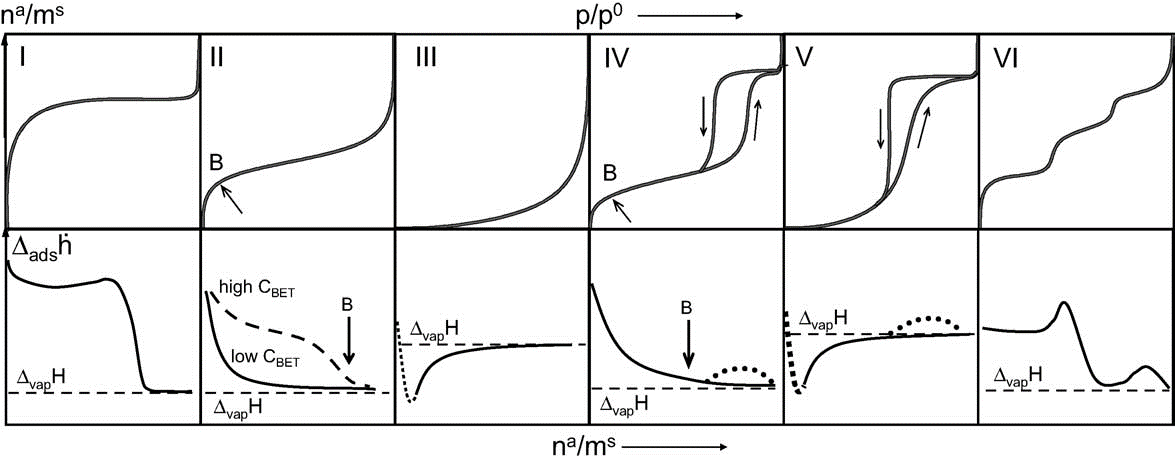
\includegraphics[width=\linewidth]{enthalpy-curves}
	\caption{
		Generalized curves of differential enthalpy of adsorption with
		respect to coverage corresponding to different
		IUPAC-defined isotherm types.
		Adapted from \citeauthor{llewellynGasAdsorptionMicrocalorimetry2005}%
		\cite{llewellynGasAdsorptionMicrocalorimetry2005}.
	}%
	\label{calo:fig:enthalpy-iupac-iso}

\end{figure}
